\documentclass[a4paper,12pt]{article}
\usepackage[T2A]{fontenc}
\usepackage[utf8x]{inputenc}
\usepackage[english,russian]{babel}
\usepackage{amssymb,amsfonts,amsmath,mathtext}
\usepackage[unicode]{hyperref}
\usepackage{listings}
\usepackage{graphicx}
\graphicspath{{images/}}
\newcommand{\anonsection}[1]{\section*{#1}\addcontentsline{toc}{section}{#1}}

\begin{document}

% Титульный лист

\begin{titlepage}
\newpage

\begin{center}

\textit{Министерство науки и высшего образования Российской Федерации \\ 
Федеральное государственное бюджетное образовательное \\
учреждение высшего образования \\
«Московский государственный технический университет \\
имени Н.Э. Баумана (национальный исследовательский университет)» \\
(МГТУ им. Н.Э. Баумана) \\}
\hrulefill
\end{center}

\vspace{2em}

\begin{flushleft}
ФАКУЛЬТЕТ <<Информатика и системы управления>> \\
\vspace{0.5em}
КАФЕДРА <<Программное обеспечение ЭВМ и информационные технологии>>
\end{flushleft}


\vspace{8em}

\begin{center}
\LARGE Лабораторная работа №2 \\
\end{center}

\vspace{1.5em}

\begin{center}
\textsc{Умножение матриц}
\end{center}

\vspace{6em}

\begin{center}
Головнев Н.В.

\vspace{4em}

ИУ7-54Б
\end{center}

\vspace{\fill}

\begin{center}
Москва 2019
\end{center}

\end{titlepage}

\tableofcontents

% Введение

\newpage
\anonsection{ВВЕДЕНИЕ}

\begin{flushleft}
Цель данной лабораторной работы:\\
% Вставь сюда цель лабораторной работы
Постановка задачи:\\
\begin{enumerate}
\item Реализовать классический алгоритм умножения матриц
\item Реализовать алгоритм умножения матриц методом Винограда
\end{enumerate}
\end{flushleft}

% Аналитическая часть

\newpage
\section{АНАЛИТИЧЕСКАЯ ЧАСТЬ}
\subsection{Описание алгоритмов}
\textit{Матрица} (matrix) представляет собой прямоугольный массив чисел.
Например, матрица А может выглядеть следующим образом:
\begin{center}
\begin{equation}
A = \left(
\begin{array}{lll}
a_{11} & a_{12} & a_{13} \\
a_{21} & a_{22} & a_{23}
\end{array}
\right) = \left(
\begin{array}{lll}
1 & 2 & 3 \\
4 & 5 & 7
\end{array}
\right)
\end{equation}
\end{center}
Матрица $A$ является матрицей размера $2 × 3 A = (a_{ij})$, где $i$ = 1,2 и $j$ = 1,2,3. Элемент на пересечении i-й строки и j-го столбца матрицы $a_{ij}$.Мы используем заглавные буквы для обозначения матриц, а их элементы обозначаются соответствующими строчными буквами с нижними индексами. Множество всех матриц размером $m×n$, элементами которых являются действительные числа, обозначается как $R^{m×n}$.В общем случае множество матриц размером $m × n$, элементы которых принадлежат множеству $S$, обозначается как $S^{m×n}$ .\\
\textit{Вектор} (vector) представляет собой одномерный массив чисел. Например,
\begin{center}
\begin{equation}
x = \left(
\begin{matrix}
2 \\
3 \\
5 \\
\end{matrix}
\right)
\end{equation}
\end{center}
\textit{Матричное умножение} (matrix multiplication) определяется следующим образом. Матрицы $A$ и $B$ могут быть перемножены, если они совместимы (compatible) в том смысле, что число столбцов $A$ равно числу строк $B$ (в общем случае выражение, содержащее матричное произведение $AB$, всегда подразумевает совместимость матриц $A$ и $B$). Если $A$ = ($a_{ij}$) — матрица размером $m × n$, а $B$ = ($b_{ij}$) — матрица размером $n × p$, то их произведение $C$ = $AB$ представляет собой матрицу $C$ = ($c_{ij}$) размером $m × p$, элементы которой определяются уравнением:
\begin{equation}
c_{ik} = \sum \limits_{j=1}^{n} a_{ij}b_{jk}
\end{equation}
для $i$ = 1, 2, . . . , $m$ и $k$ = 1, 2, . . . , $p$. \\
\\
Если посмотреть на результат умножения двух матриц, то видно, что каждый элемент в нем представляет собой скалярное произведение соответствующих строки и столбца исходных матриц. Можно заметить также, что такое умножение допускает предварительную обработку, позволяющую часть работы выполнить заранее. \\
Рассмотрим два вектора: $V = (v_1, v_2, v_3, v_4)$ и $W = (w_1, w_2, w_3, w_4)$. Их скалярное произведение равно:
\begin{center}
\begin{equation}
V × W = v_1w_1 + v_2w_2 + v_3w_3 + v_4w_4.
\end{equation}
\end{center}
Это равенство можно переписать в виде:
\begin{center}
\begin{equation}
V × W = (v_1 + w_2)(v_2 + w_1) + (v_3 + w_4)(v_4 + w_3) - v_1v_2 - v_3v_4 - w_1w_2 - w_3w_4.
\end{equation}
\end{center}
Кажется, что второе выражение задает больше работы, чем первое: вместо четырех умножений мы насчитываем их шесть, а вместо трех сложений - десять. Менее очевидно, что выражение в правой части последнего равенства допускает предварительную обработку: его части можно вычислить заранее и запомнить для каждой строки первой матрицы и для каждого столбца второй. На практике это означает, что над предварительно обработанными элементами нам придется выполнять лишь первые два умножения и последующие пять сложений, а также дополнительно два сложения. 

\newpage
\subsection{Вывод}
% Придумай что-нибудь 

% Конструкторская часть

\newpage
\section{КОНСТРУКТОРСКАЯ ЧАСТЬ}

\subsection{Разработка алгоритмов}
На вход у всех алгоритмов передаются в качестве параметров:
\begin{enumerate}
\item Указатели на перемножаемые матрицы;
\item Размеры матриц;
\item Указатель на матрицу, в которую будут сохранены результаты умножения;
\item В алгоритме Винограда в качестве параметров добавляются ещё 2 указателя на массивы заранее вычисленных произведений.
\end{enumerate}
Возвращаемое значение: код ошибки (0 в случае успеха, иначе отрицательное значение). \\
Побочные эффекты: изменяются значения в матрице результата.

\newpage
\subsection{Схемы алгоритмов}
Ниже приведены схемы стандартного алгоритма умножения матриц\\(Рис. 1) и алгоритма Винограда умножения матриц(Рис. 2-3).
\begin{figure}[h!]
\center{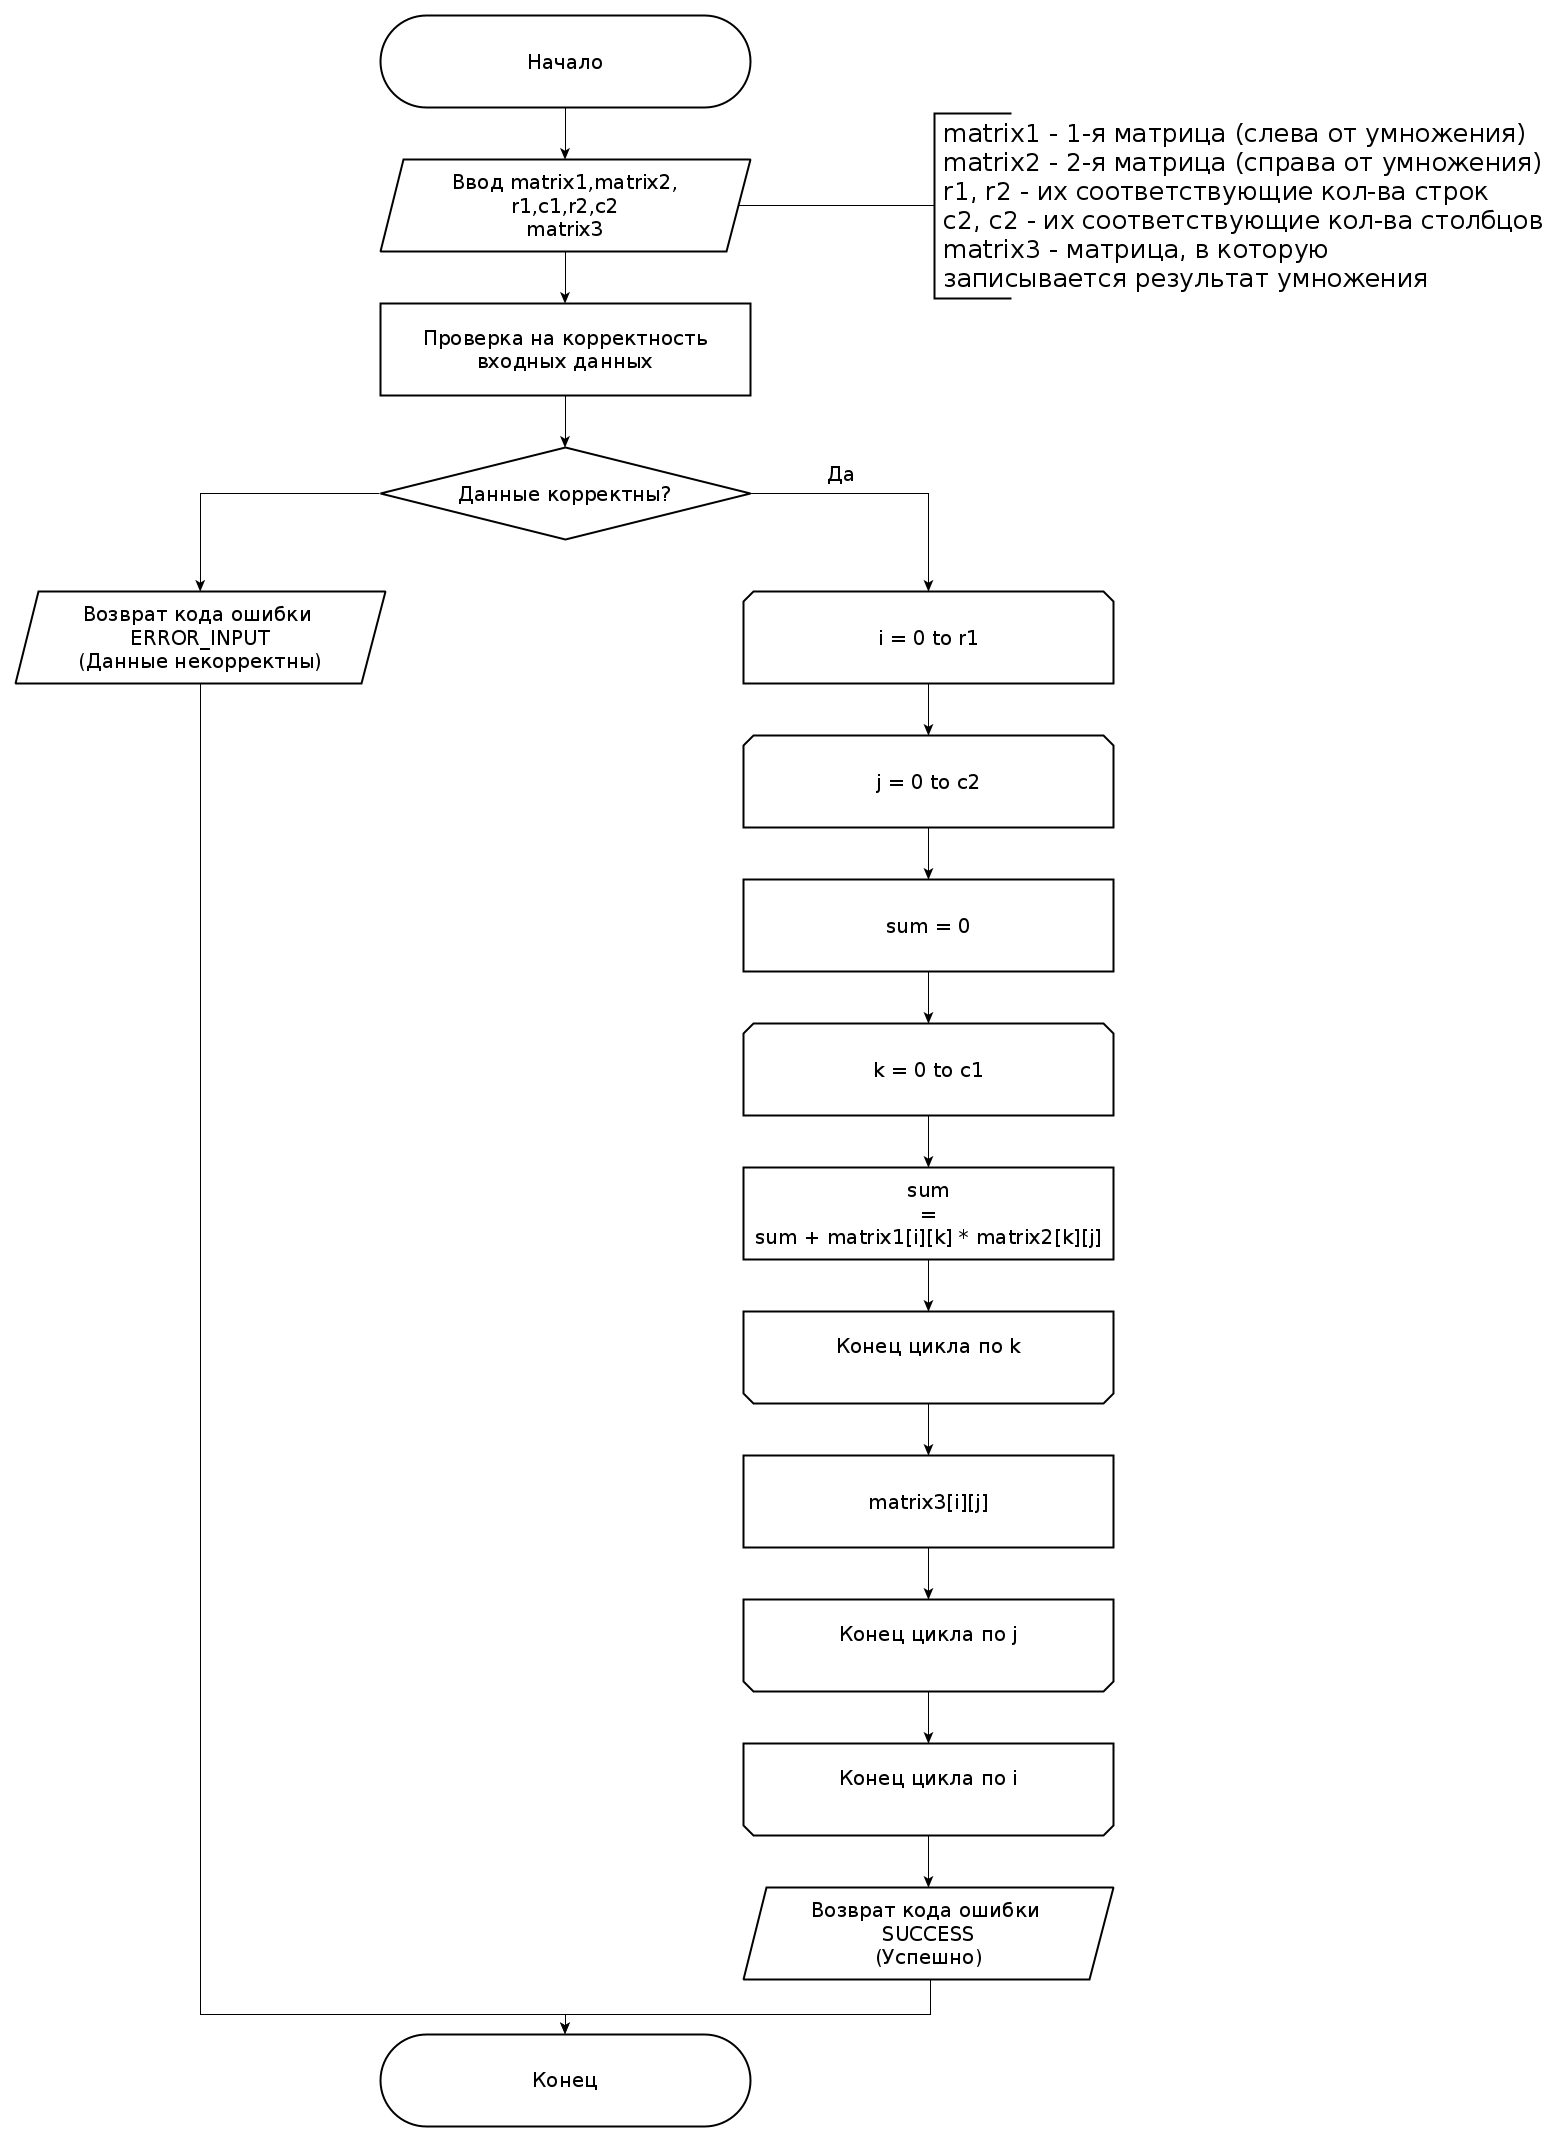
\includegraphics[scale=0.2]{multiply_standard.png}}
\caption{Схема стандартного алгоритма умножения матриц}
\label{images:multiply_standard}
\end{figure}

\begin{figure}[p]
\center{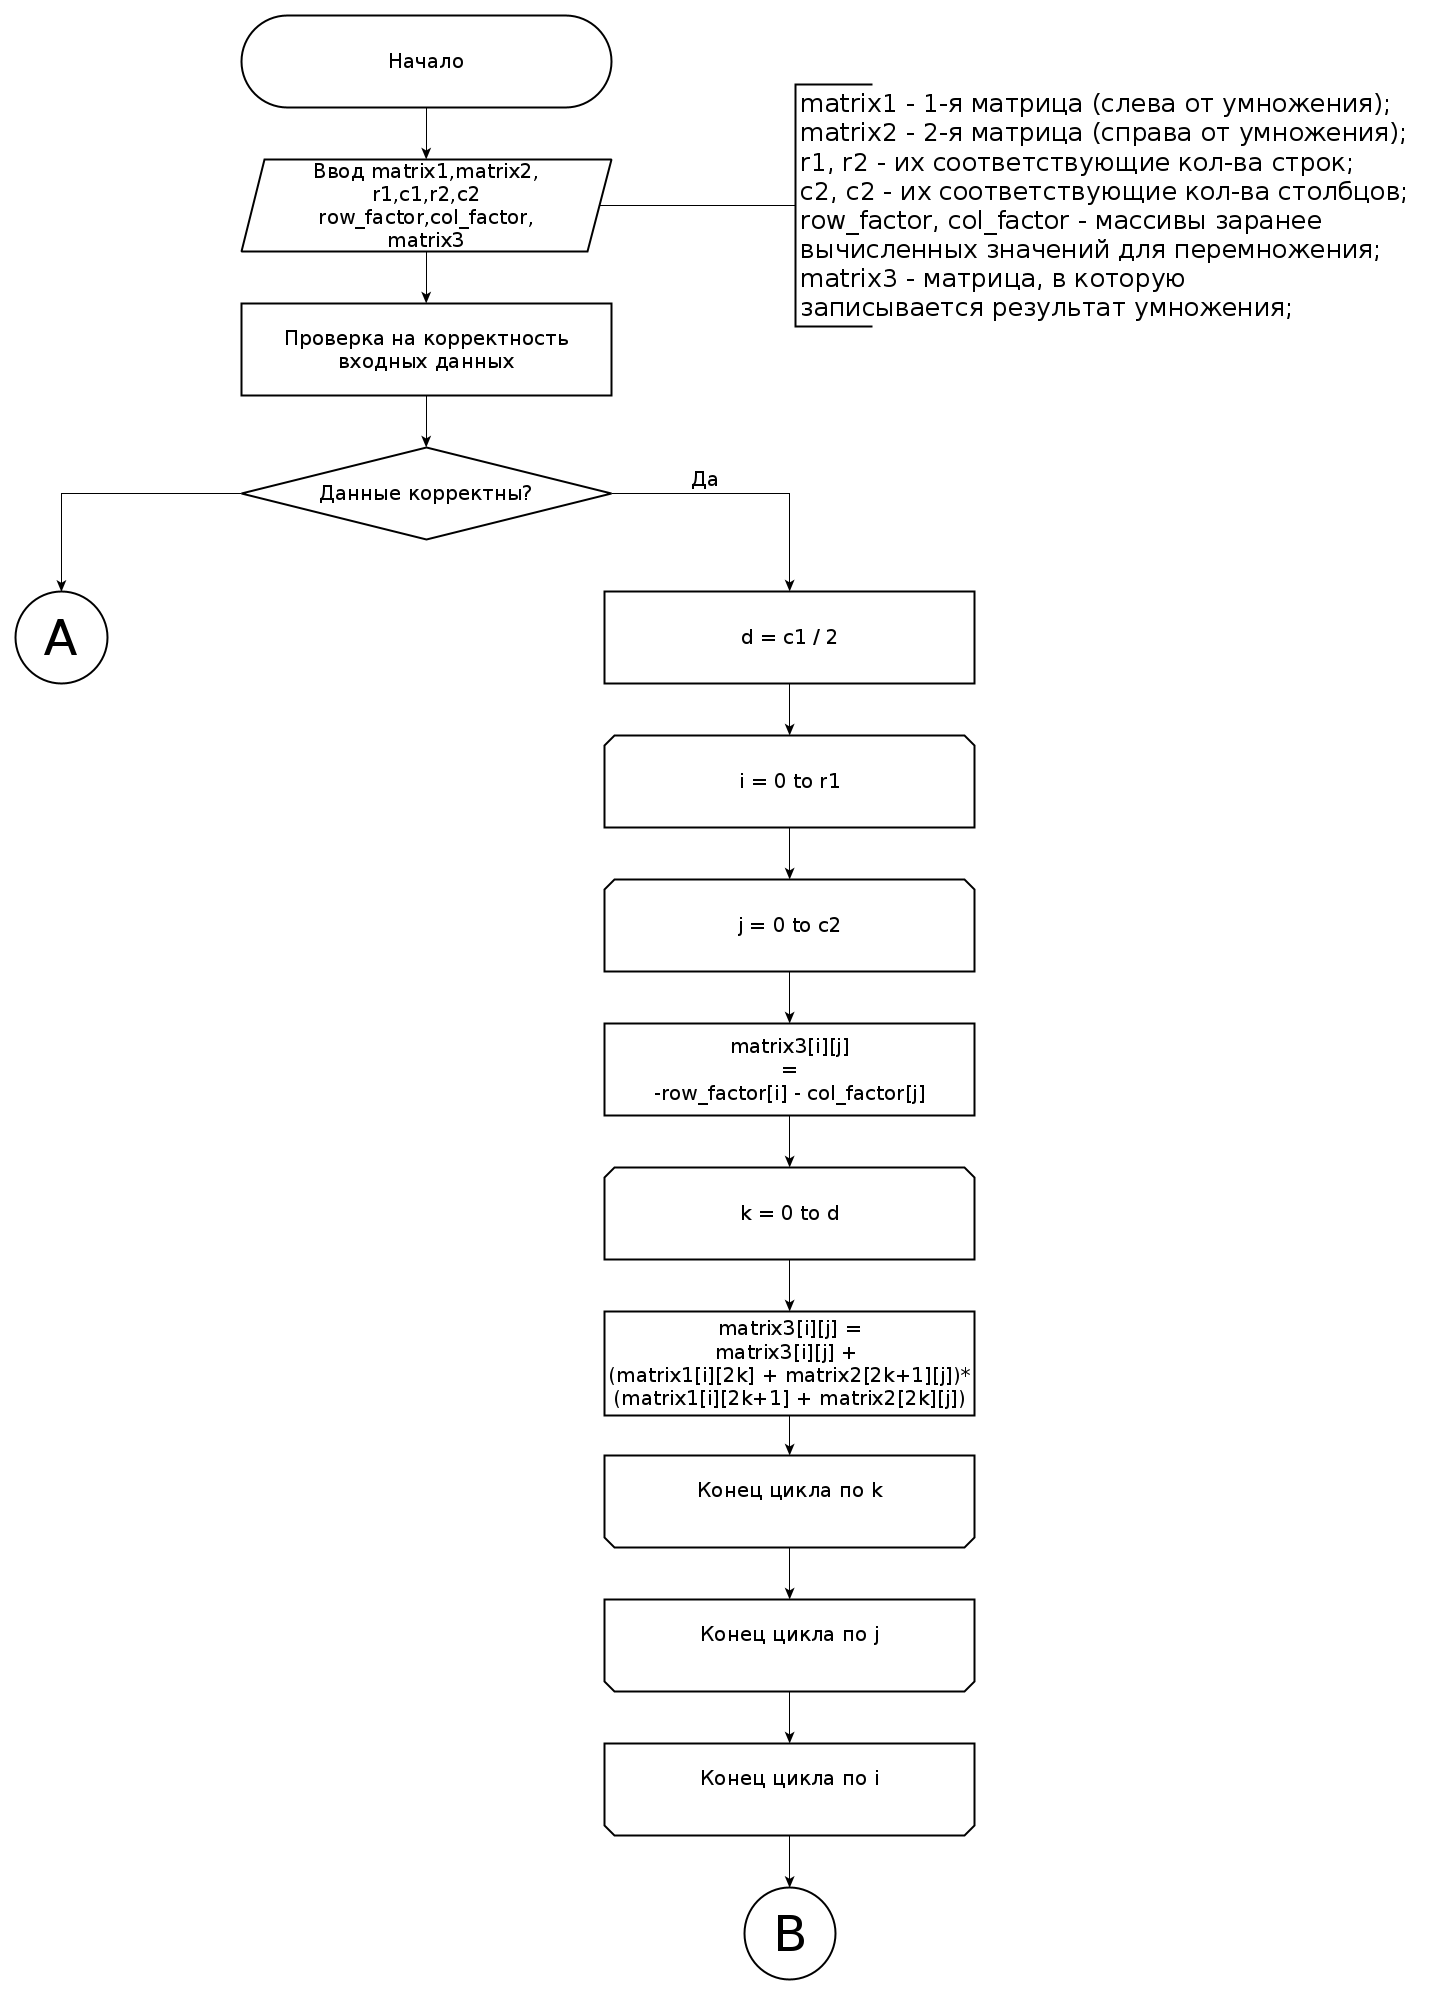
\includegraphics[scale=0.25]{multiply_vinograd1.png}}
\caption{Схема алгоритма Винограда умножения матриц(Начало)}
\label{images:multiply_vinograd1}
\end{figure}

\begin{figure}[p]
\center{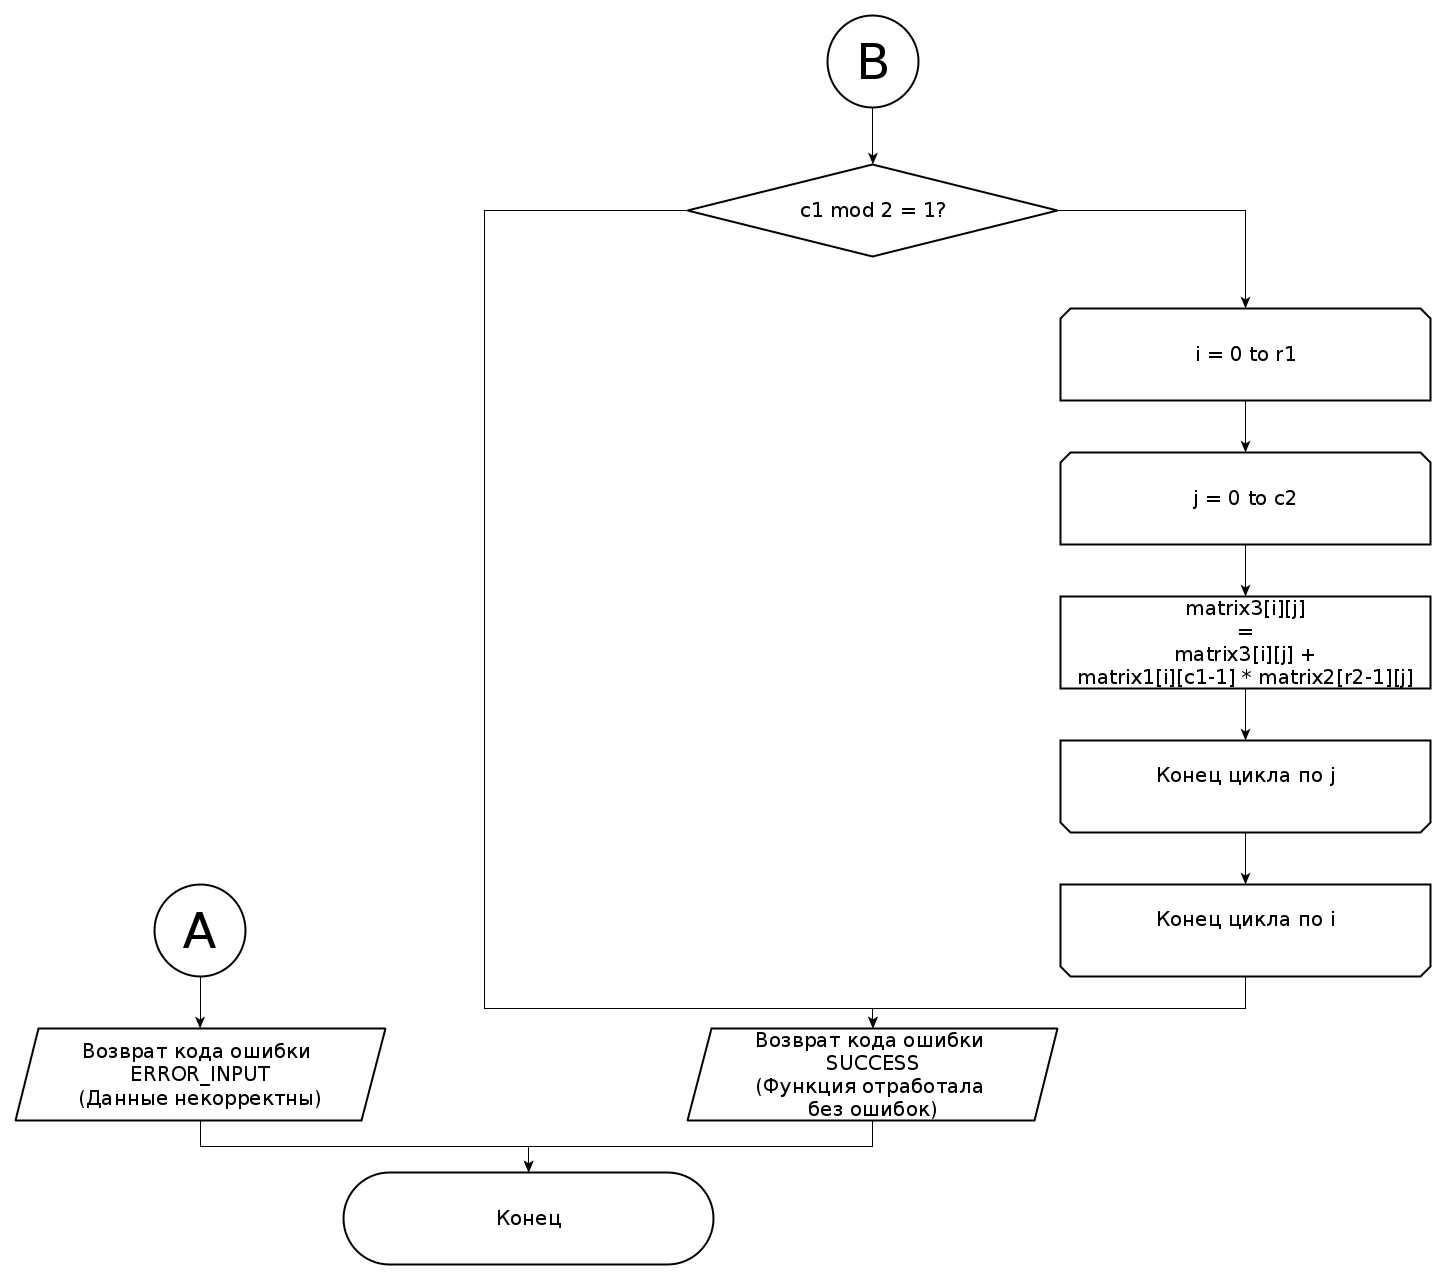
\includegraphics[scale=0.25]{multiply_vinograd2.png}}
\caption{Схема алгоритма Винограда умножения матриц(Конец)}
\label{images:multiply_vinograd2}
\end{figure}
% Как же я ненавижу делать эти схемы

\newpage
\subsection{Вывод}
% Для начала надо сделать предыдущее

\newpage
\section{ТЕХНОЛОГИЧЕСКАЯ ЧАСТЬ}
\subsection{Требования к программному обеспечению}

\begin{flushleft}
Программа должна работать на операционной системе Arch Linux. Программа должна
содержать 2 режима:
\begin{itemize}
\item Пользовательский
\item Экспериментальный
\end{itemize}
В пользовательском режиме пользователь должен иметь возможность вводить матрицы и получать на выходе результаты работ всех реализованных алгоритмов умножения матриц. В экспериментальном режиме засекается процессорное время работы каждого алгоритма, результаты записываются в отдельные файлы. Впоследствии данные из этих файлов можно вывести в виде графика зависимости процессорного времени от размеров матриц.
\end{flushleft}

\newpage
\subsection{Средства реализации}
Для реализации данных алгоритмов был выбран язык программирования С, компилятор
gcc и некоторые функции из библиотеки glibc (memcpy, malloc и тд...). \\
Удобства, предоставляемые языком C:
\begin{itemize}
\item Прямой доступ к памяти;
\item Возможность составлять простейшие структуры данных;
\end{itemize}
Для вывода графиков использовался Python3 (библиотека Matplotlib)

\newpage
\subsection{Листинг кода}
Ниже приведены реализации алгоритмов на С.\\
\lstdefinestyle{customc}{
  belowcaptionskip=1\baselineskip,
  breaklines=true,
  frame=L,
  xleftmargin=\parindent,
  language=C,
  showstringspaces=false,
  basicstyle=\footnotesize\ttfamily
}

% В директории надо добавить листинги с кодом
\lstinputlisting[captionpos=b, caption=\label{listings:listing1}Реализация стандартного алгоритма умножения матрица(\ref{images:multiply_standard}), style=customc]{listing1.c}
\newpage
\lstinputlisting[captionpos=b, caption=\label{listings:listing2}Реализация алгоритма умножения матриц Винограда(\ref{images:multiply_vinograd1}), style=customc]{listing2.c}

\newpage
\subsection{Вывод}
Используя язык программирования C, в ходе практической работы были спроектированы и написаны реализации алгоритмов умножения матриц. Используя эти реализации были написаны 2 приложения: пользовательское приложение и приложение для подсчета процессорного времени выполнения этих алгоритмов.

\newpage
\section{ЭКСПЕРИМЕНТАЛЬНАЯ ЧАСТЬ}
\subsection{Характеристики аппаратного и программного обеспечения}
\flushleft{Тестирование приложения проводилось на машине со следующими характеристиками:\\}
\begin{itemize}
\item Процессор Intel® Core™ i7-7700HQ;
\item Оперативная память 16 ГБ;
\item Операционная система - Arch Linux с рабочим окружением Gnome 3.
\end{itemize}

\newpage
\subsection{Примеры работы}
\begin{flushleft}
На Рис., предсавленном ниже, демонстрируется работа приложения. Запуск приложения осуществляется из эмулятора терминала в Arch Linux. Во время работы приложение запрашивает у пользователя ввод параметров матриц, а также ввод отдельных строк каждой матрицы. На выходе она печатает
\end{flushleft}
\begin{figure}[h]
\center{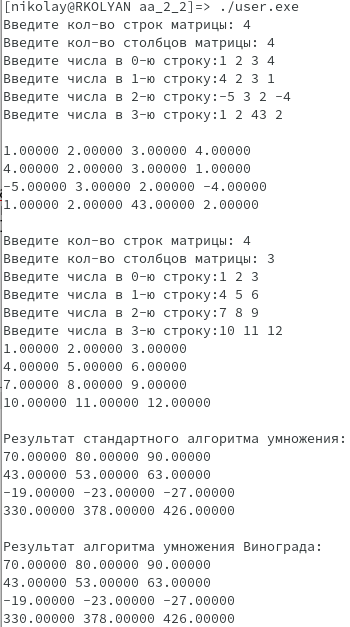
\includegraphics[scale=0.6]{example.png}}
\caption{Пример работы приложения}
\label{images:example}
\end{figure}

\newpage
\subsection{Результаты тестирования}

\begin{table}[h]
\caption{\label{tablice:tests}Результаты тестирования приложения}
\begin{center}
\begin{tabular}{|c|c|c|c|}
\hline
1-я матрица & 2-я матрица & стандартное умножение & умножение Винограда \\
\hline
3 & 4 & 12 & 12 \\
\hline
1 2 & 5 & & \\
 & -6 & -9 & -9 \\
\hline
1 2 & 3 4 & 5 8 & 5 8 \\
3 4 & 1 2 & 13 20 & 13 20 \\
\hline
1 2 3 & 1 1 1 & 14 14 14 & 14 14 14 \\
1 2 3 & 2 2 2 & 14 14 14 & 14 14 14 \\
      & 3 3 3 & & \\
\hline
1 1 1 & 1 2 3 & 3 6 9 & 3 6 9 \\
2 2 2 & 1 2 3 & 6 12 18 & 6 12 18 \\
3 3 3 & 1 2 3 & 9 18 27 & 9 18 27 \\
\hline
\end{tabular}
\end{center}
\end{table}

% Не знаю как, но нужно здесь показать небольшие результаты тестирования.

\newpage
\subsection{Постановка эксперимента по замеру времени}
\begin{flushleft}
Для вычисления процессорного времени работы алгоритмов использовалась функция clock(), объявленная в заголовочном файле time.h из библиотеки glibc. \\
Требования к программе, считающей время выполнения алгоритмов:
\begin{itemize}
\item Ввод пользователем таких параметров, как:
\begin{itemize}
\item Максимальная длина стороны обоих матриц;
\item Кол-во итераций на каждый рассматриваемый случай (для высчитывания среднего значения);
\end{itemize}
\item Матрицы генерируются со случайными числами;
\item Результаты вычислений должны сохранятся в текстовых файлах.
\end{itemize}
\end{flushleft}

\newpage
\subsection{Сравнительный анализ на материале экспериментальных данных}
Ниже представлен график зависимости времени работы алгоритмов умножений матриц. Из полученных данных видно, что алгоритм умножения Винограда уступает стандартному умножению у квадратных матриц с размерами <= 800x800. Начиная приблизительно с интервала 800×800-900×900, алгоритм Винограда работает наравне, а то и вовсе быстрее стандартного.
\begin{figure}[h!]
\center{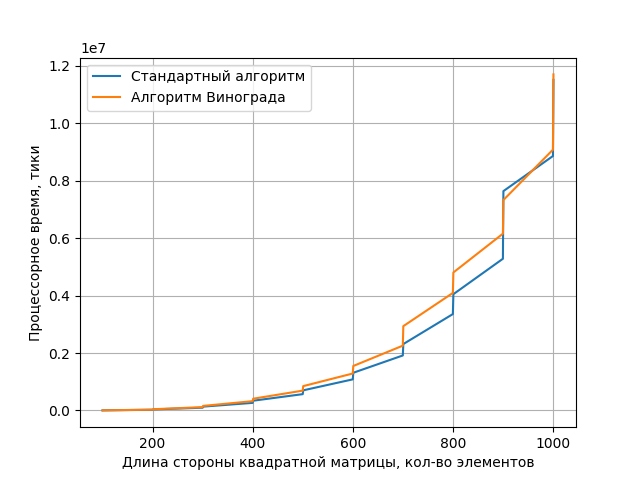
\includegraphics[scale=1]{graphics.png}}
\caption{График зависимости времени работы алгоритмов от длин сторон матриц}
\label{images:graphics}
\end{figure}

\newpage
\subsection{Оценка затрачиваемой памяти}
1)Размер затрачиваемой динмачески выделенной памяти на стандартный алгоритм умножения (в байтах):
\begin{center}
\begin{equation}
M_1 = D(2r_1 + r_2)  + t(r_1c_1 + r_2c_2 + r_1c_2)
\end{equation}
\end{center}
где \\
$D$ - размер дескриптора каждой строки,\\
$t$ - размера выбранного для элементов матрицы типа данных,\\
$r_1, r_2$ - количества строк в матрицах 1 и 2 соответственно,\\
$c_1, c_2$ - количества столбцов в матрицах 1 и 2 соответственно.\\
Размер памяти, выделенной под стек $M_2 = 56$.
В итоге размер всей используемой памяти:
\begin{center}
\begin{equation}
M_s = D(2r_1 + r_2)  + t(r_1c_1 + r_2c_2 + r_1c_2) + 56
\end{equation}
\end{center}
2)Размер затрачиваемой динмачески выделенной памяти на стандартный алгоритм умножения (в байтах):
\begin{center}
\begin{equation}
M_v = D(2r_1 + r_2)  + t(r_1c_1 + r_2c_2 + r_1c_2 + c_1 + r_2)
\end{equation}
\end{center}
где \\
$D$ - размер дескриптора каждой строки,\\
$t$ - размера выбранного для элементов матрицы типа данных,\\
$r_1, r_2$ - количества строк в матрицах 1 и 2 соответственно,\\
$c_1, c_2$ - количества столбцов в матрицах 1 и 2 соответственно.\\
Размер памяти, выделенной под стек $M_2 = 68$.
В итоге размер всей используемой памяти:
\begin{center}
\begin{equation}
M = D(2r_1 + r_2)  + t(r_1c_1 + r_2c_2 + r_1c_2 + c_1 + r_2) + 68
\end{equation}
\end{center}
Сравнивая (7) и (9) следует, что реализация алгоритма Винограда умножения матриц требует больше памяти, чем стандартный алгоритм умножения. \\
Процентное отношение:\\
\begin{center}
\begin{equation}
\eta = \frac{M_s}{M_v} = 1 - \frac{(c_1 + r_2)t + 12}{D(2r_1 + r_2)  + t(r_1c_1 + r_2c_2 + r_1c_2 + c_1 + r_2) + 68}
\end{equation}
\end{center}
\newpage
\subsection{Вывод}
Стандартный алгоритм умножения матриц всегда эффективнее алгоритма Винограда по памяти. Что касается сравнения эффективности по скорости умножения, то стандартный алгоритм работает быстрее на размерах матриц до 800x800 - 900x900,
При больших матрицах алгоритм Винограда работает практически наравне или даже быстрее стандартного.

\newpage
\anonsection{ЗАКЛЮЧЕНИЕ}
% Нужно написать и эту каку



\newpage
\anonsection{СПИСОК ИСТОЧНИКОВ}
\begin{itemize}
\item Кормен, Томас Х., Лейзерсон, Чарльз И., Ривест, Рональд Л., Штайн, Клифорд. Глава 28. Работа с матрицами // Алгоритмы: построение и анализ = Introduction to Algorithms. — 2-e издание. — М.: «Вильямс», 2005. — С. 833 - 839. — ISBN 5-8459-0857-4.
\item http://www.algolib.narod.ru/Math/Matrix.html
\end{itemize}
% ХЗ что ещё брать кроме ХАБРа

\end{document}
